\section{Black Hole Fundamental Plane in Illustris}

\label{sec:analysis}Starting with our sample of black holes from
the Illustris simulation, we seek a relation between the masses and
accretion rates. This relation allows us to construct a power-law
relationship between $M$ and $\dot{M}$ using linear least-squares
(Figure \ref{fig:bhpop_hist2d}). The best-fit is given by

\begin{equation}
\log\dot{M}=0.869\log M_{BH}-17.855.\label{eq:int_relation}
\end{equation}
This relationship reflects the intrinsic properties of the simulation,
and is independent of any models.
\begin{figure}
\centering{}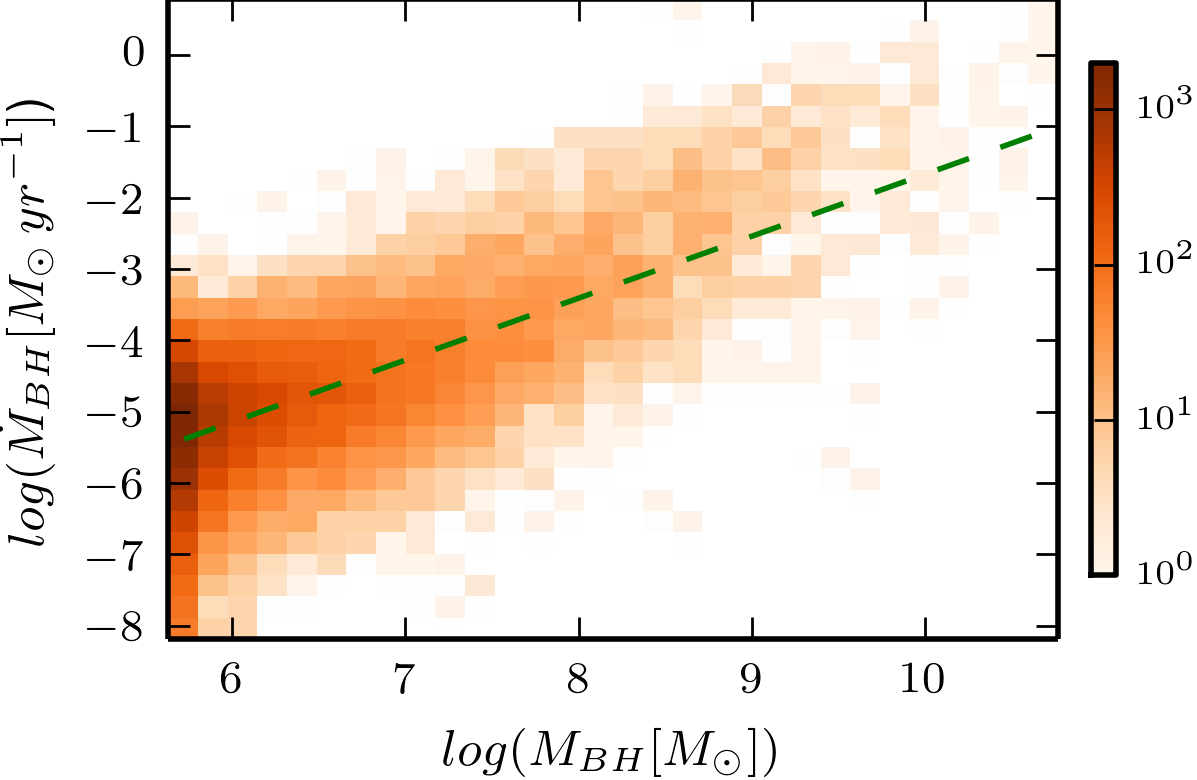
\includegraphics[clip]{Figures/Illustris2_bhpop_hist2d}
\protect\caption{\label{fig:bhpop_hist2d}Black hole accretion rate as a function of
black hole mass for the Illustrist-2 simulation for our sample. The
best-fit power-law relationship between $M$ and $\dot{M}$ is shown
in green. Colors correspond to a two-dimensional density of the same
plot sampled in log space.}
\end{figure}

The fundamental plane of black holes in the local universe from M03
is shown in Figure \ref{fig:Fp} and defined as

\begin{equation}
\log L_{R}=0.6\log L_{x}+0.78\log M_{BH}+7.33
\end{equation}
where the $L_{R}$ is the radio luminosity, $L_{X}$ is the X-ray
luminosity, and $M_{BH}$ is the mass of the black hole. This is expression relates different observable properties of BH and is an expression that corelates the feedback of the BH.  Never the less,  there are two more expressions that relates the intrinsic properties of the BH. This relations uses either one of the luminosities  (radio or X-ray) the mass and the accretion rate of the BH.  For the purpose of this analysis the BH relation that will be us is:

\begin{equation}
\log L_{x}=\log M+q\log\dot{M}+K\;,\label{eq:LxFP}
\end{equation}
where $K$ is a normalization constant. Depending on the accretion
flow model, the efficiency coefficient $q$ ranges from 0.5 (optically
thick thin disk accretion flow) to 2.3 (advection dominated accretion
flow). The most significant aspect of the fundamental plane is that
it is a correlation which we can apply our general knowledge of galactic
BHs to AGNs and vice versa.

\begin{figure}
\centering{}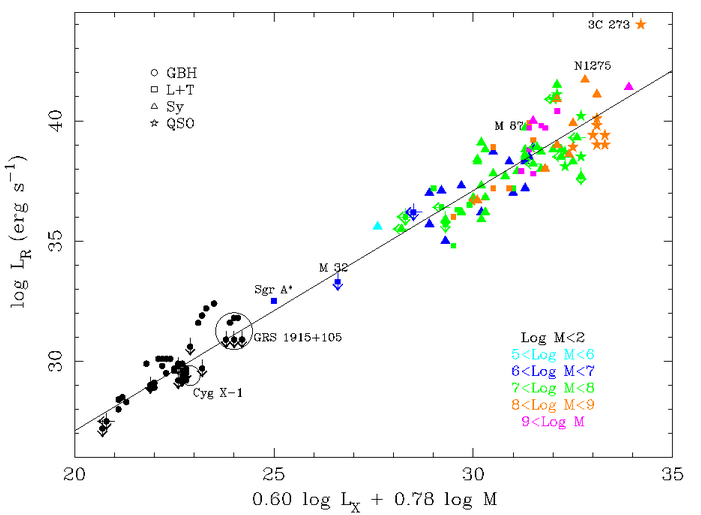
\includegraphics[clip,scale=0.35]{Figures/FP} \protect\caption{\label{fig:Fp}Edge-on view of the fundamental plane from M03 relating
the black hole mass to the radio and X-ray luminosities. Symbols indicate
the type of emission-line galaxy of the host and colors correspond
to the mass of the black hole in units of $\log\left({\rm M}_{\odot}\right)$.
Several well-known galaxies hosting an AGN are listed, as well.}
\end{figure}

In other to model and calculate the parameters in the the BH fundamental plane, a method to calculate the luminosity is needed.  This is due the fact that the luminosity in not an intrinsic property of the simulation. The calculation of the luminosity for BH can be approximated by two different models. The first one takes into account the Eddington luminosity of the BH. The second method uses the thin disk approximation. Both of these approaches for the luminosity give the bolometric luminosity. To get the X-ray luminosity from the bolometric luminosity we use the \citet{elvis1994atlasof} data sample to calculate a template.  The data contains the bolometric luminosity, the X-ray flux and the redshift for 47 BH.  The first step is to convert the flux to a luminosity by means of the redshift. The data is fit using a power law given by (\ref{fig:Elvis_template}):

\begin{equation}
L_{x}=0.1947L_{bol}+1.656\times10^{-15}\;.
\end{equation}

Considering the BHs have luminosity given by the Eddington luminosity with an efficiency of 10\% Eddington.  The 10\% efficiency is a general condition found in BH \textbf[{REFERENCE]}.  Using the Elvis Template the correlation between mass and bolumetic luminosity can be changed to mass and X-ray luminosity given by:

\begin{equation}
L_{x}=623.04M+1.656\times10^{-15}\;.\label{eq:Lx_propto_m}
\end{equation}

The second model consider the luminosity mechanism to be proportional
to a thin disk accretion. For this case the efficiency is allso  10\% and that will be the case use in all the BH.  The thin disk luminosity relates the luminosity to the accretion rate.  Using the Elvis template the X-ray luminosity is express in terms of the accretion rate by:

\begin{equation}
L_{x}=4.64\times10^{19}\dot{M}+1.656\times10^{-15}\;,\label{eq:Lx_propto_mdot}
\end{equation}

for all the cases the masses, accretion rates and luminosities are
measured in $M_{\odot}$, $M_{\odot}s^{-1}$ and $L_{\odot}$. With
equations \ref{eq:Lx_propto_m} and \ref{eq:Lx_propto_mdot} and using
the equation \ref{eq:LxFP}. The fundamental plane equation can be
rewritten in terms of mass, accretion rate, k and q. By means of using
the intrinsic mass to accretion relation, equation \ref{eq:int_relation},
the fundamental plane can be expressed with only 3 variables \textbf{which 
three variables?}


\begin{figure}
\centering{}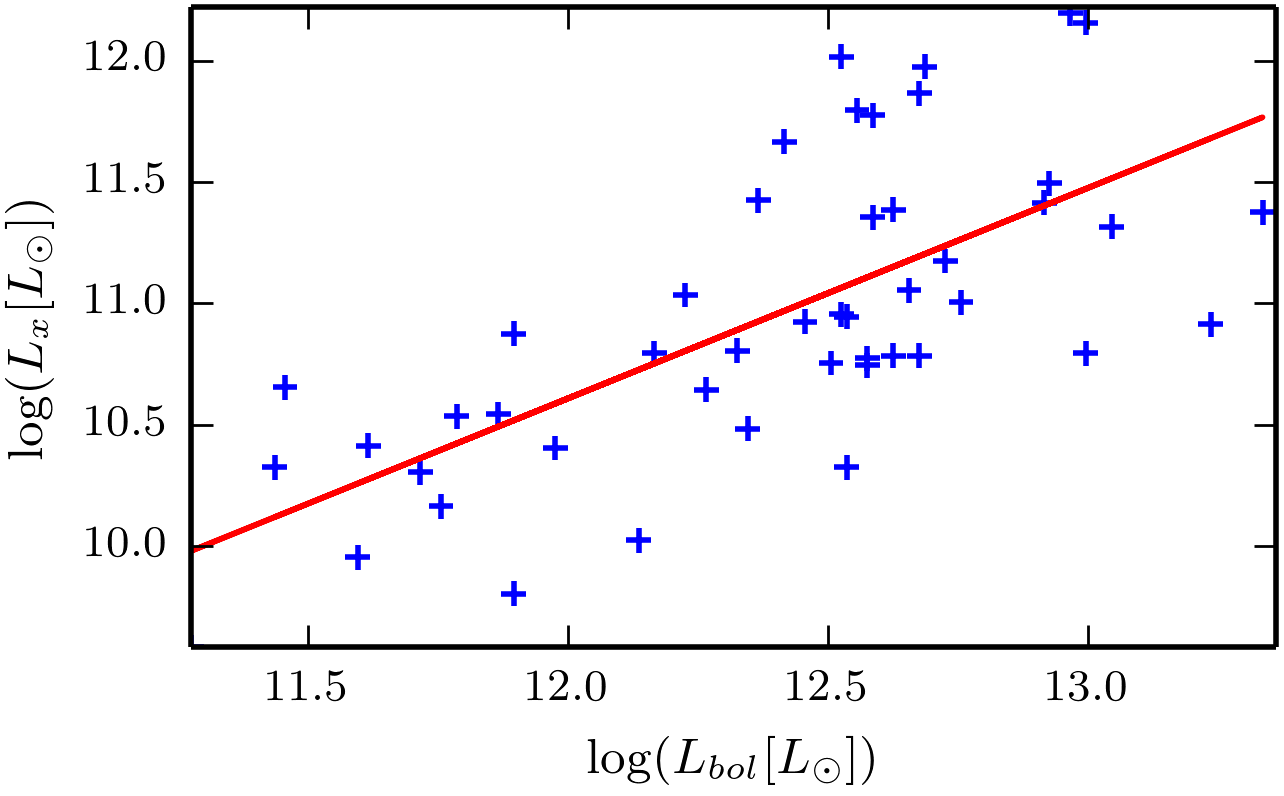
\includegraphics[clip]{Figures/elvis_template} \protect\caption{\label{fig:Elvis_template}The data points from the BH luminosities
over plot with the best-fit linear relation between $L_{x}$ and $L_{bol}$
for the sample.}
\end{figure}
\begin{figure}
\begin{centering}
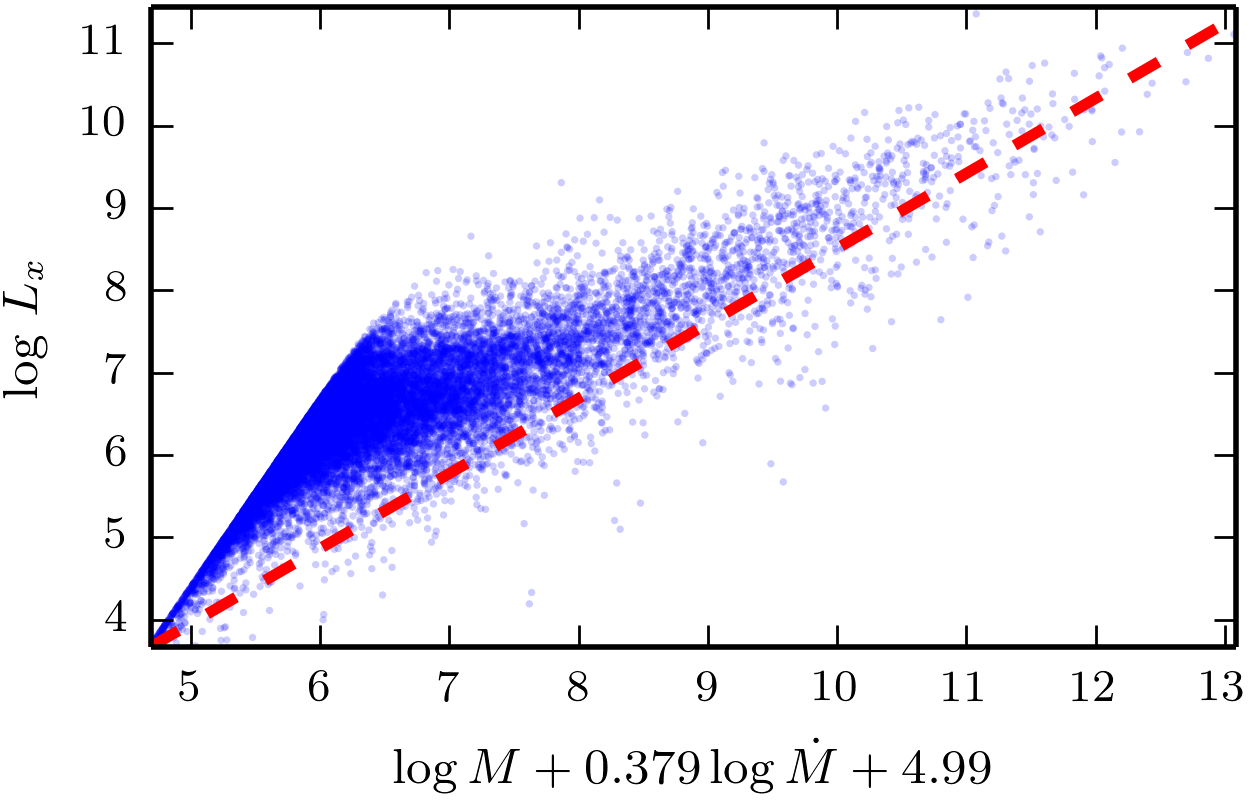
\includegraphics{Figures/fp_fit}
\par\end{centering}

\protect\caption{\label{fig:q_nr_hist}The fit to the fundamental plane
$\log\left(L_x\,[L_\odot]\right) = \log M+0.378\log\dot{{M}}+9.47$ using our sample. The
X-ray luminosities are in units of $L_\odot$, the masses in units of $M_\odot$, and the
accretion rate in units of $M_{\odot}\,s^{-1}$.}
\end{figure}
